\chapter{Framework}

% **************************** Define Graphics Path **************************
\ifpdf
    \graphicspath{{Chapter3/Figs/Raster/}{Chapter3/Figs/PDF/}{Chapter3/Figs/}}
\else
    \graphicspath{{Chapter3/Figs/Vector/}{Chapter3/Figs/}}
\fi
The chapter aims to present the basic framework for our vessel segmentation algorithm.
The chapter is divided into 4 parts. In the first part we discuss the basic framework of our algorithm. Part 2 and Part3 talk about the various preprocessing methods and how the methods was applied to our problem.
\section{Vessel segmentation Framework}
The image segmentation framework takes as its input a list of fundus images, $I = (I^{(1)},I^{(2)}....., I^{(n)} )$  and their correspoding ground truth segmentation maps  $S = (S^{(1)},S^{(2)}....., S^{(n)} )$. The fundus images $I^n$ can be grayscale or RGB color images. For each n, $S^n$ ,the binary segmentation map is of the same size as of $I^n$. For a given fundus image, $I^n$, let $I^n(x,y)$ denote the pixel value at position (x,y) and $S^n(x,y)$ denotes the corresponding pixel in the segmentation map $S^n$. The pixels in segmentation map take either a value of 1 or 0 denoting the presenece or absence of vessel respectively.

\begin{figure}
	\centering
	\begin{subfigure}[b]{0.45\textwidth}
		\centering
		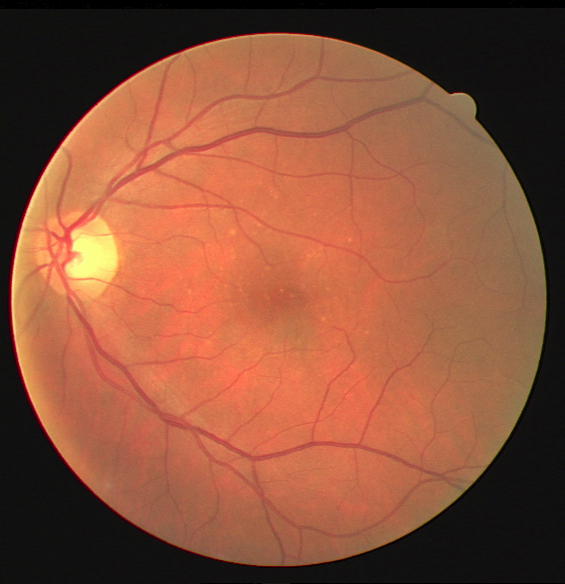
\includegraphics[width=\textwidth]{fundusimage}
		\caption{Fundus Image}
		\label{fig:fundusex}
	\end{subfigure}
	\hfill
	\begin{subfigure}[b]{0.45\textwidth}
		\centering
		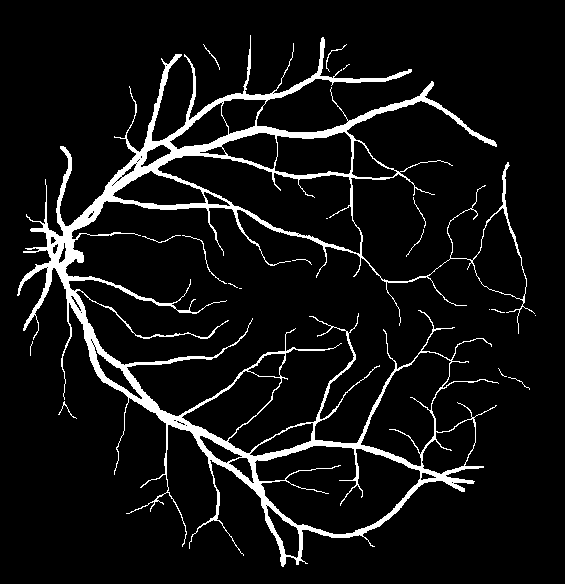
\includegraphics[width=\textwidth]{fundusimageseg}
		\caption{Segmented Vessels}
		\label{fig:fundusex seg}
	\end{subfigure}
	\caption{Fundus Image and its segmentation}
	\label{fig:fundus example}
\end{figure}


For clarity and simplicity, the fundus images will be referred as I and the corresponding segmentation image as S. Fig~\ref{fig:fundus example} shows an example of fundust image on the left and the correspoding segmentation image on the right.

In this thesis we aim to develop methods that use the training data I and S to learn a predictor that segments the vessels in new unseen fundus images.The proposed problem is solved in a patch based framework, in which we decompose each image into smaller images (called as patches) centered around each pixel of the original image. Thus a given fundus image I and segmentation map S can be represented in terms of their patches as 
\begin{gather}
I = \{ P^I_{x,y} \}  \\
S = \{ P^S_{x,y} \} 
\end{gather}
where $P^I_{x,y}$ and $P^S_{x,y}$ represent a $w $ x $ w$ patch centered at pixel (x,y) of I and S respectively.

The training set I \& S is composed of such small patches and a classifier is trained which learns a set of patches 

\subsection{Preprocessing}
In our task we have explored some of the preprocessing steps including Patch Normalization, Contrast streteching, Local contrast nomralization.

All the input patches are normalizaed by subtracting the mean and standard deviation per patch. In addition to this we also test with normalizing the entire image before patch generation.

In some of the experiments, we improve the image contrast by utilizing Contrast Limited Adaptive Histogram Equalization (CLAHE) as explained in section{}.

In our task we have explored some of the preprocessing steps including Patch Normalization, Contrast streteching, Local contrast nomralization.

All the input patches are normalizaed by subtracting the mean and standard deviation per patch. In addition to this we also test with normalizing the entire image before patch generation.

In some of the experiments, we improve the image contrast by utilizing Contrast Limited Adaptive Histogram Equalization (CLAHE) as explained in section{}.

Rotations
To provide for rotational invariance and learn better representatives, rotated patches are also included in our learning phase. Each of the training images are additionaly rotated at angles of 30,60,90 and patches are calculated.

\section{Datasets}
For testing the performance of our algorithm , we train and test our system on the following publically available datasets. In this section we describe the characteristics of these datsets

\subsection{DRIVE}
The Digital Retinal Images for Vessel Extraction (DRIVE) dataset consists of 40 color retinal images randomly selected from diabetic retinopathy screening program for 400 diabetic patients.Each of these images in dataset are JPEG compressed and have a dimensions of 768 x 584 pixels captured at a resolution on bits per pixel. The images are captures with a 45degree field of view (FOV).
Of the 40 images in the datset, 7 show sign of diabetic retinopathy , while the remaining 33 do not consist of any pathology. Each image is provided with a corresponding mask delineating the FOV.

The dataset is divided is provided with divisions in terms of training and testing set, with each set consisting of 20 images. Each of the 40 images have been manually segmented by human observers trained by an experienced optamologist. For the training set, single ground truth segmentation of the vessels is provided. The test set is provided with two ground truth segmentations, of which the first one is used as gold standard and the other is used to compare the performance with an independent human observer.

\subsection{STARE}
The STARE dataset consists of 20 images with blood vessel segmentations, out of which 10 show signs of pathology. The images have been capture with a FOV of 35degrees at 8 bit per pixel resolution, with dimesnsions of each image as 605 x 700 pixels. The dataset consists of segmentation provided by two human observers. In our experiements, we consider the segmentations provided by the first observer as ground truth.

For the experiements, the dataset is randomly divided into training and test sets each consisting of 10images.

\subsection{HRF}
he High Resolution Fundus (HRF) image databse consists of 45 images of which 15 images come from healthy patients , 15 from patients with diabetic retinopathy and 15 of glacumatous patients.

The images were captured with a FOV of 60degrees, at a high resolution of 24bits per pixel. The size of each image is 3504 x 2336 pixels and stored with JPEG compression. 

Each image is provided a manual segmentation of vessesl as segmented by three independent human observers trained by experienced optahmologists.The dataset also provides a corresponging mask image of each image delineating the FOV.

\subsection{ARIA}
The ARIA dataset consists of three groups of images. One of the group consists of 92 images with age-related macular degeneration, the other with 59 images from diabetic patients and the last group with 61 images from a control group.
The images are captures with a 50degree FOV, stored in uncompressed TIFF format, with a resolution of 8bits oer pixel. Each image has dimensions of 768 x 576 pixels.

The dataset provides with blood vessel segmentation images as manually segmented by experts and a corresponding mask delinating the FOV region.



\begin{table}
\caption{Even better looking table using booktabs}
\centering
\label{table:good_table}
\begin{tabular}{l c c c c}
\toprule
\multirow{2}{*}{Dental measurement} & \multicolumn{2}{c}{Species I} & \multicolumn{2}{c}{Species II} \\ 
\cmidrule{2-5}
  & mean & SD  & mean & SD  \\ 
\midrule
I1MD & 6.23 & 0.91 & 5.2  & 0.7  \\

I1LL & 7.48 & 0.56 & 8.7  & 0.71 \\

I2MD & 3.99 & 0.63 & 4.22 & 0.54 \\

I2LL & 6.81 & 0.02 & 6.66 & 0.01 \\

CMD & 13.47 & 0.09 & 10.55 & 0.05 \\

CBL & 11.88 & 0.05 & 13.11 & 0.04\\ 
\bottomrule
\end{tabular}
\end{table}
